% 图 2.3 (a) 萘：两个稠合苯环 (b) 石墨：六角层堆叠，隔层原子对齐（竖直虚线）
\documentclass[tikz,border=5pt]{standalone}
\usetikzlibrary{arrows.meta}
\usepackage{amsmath}
\usepackage{bm}
\usepackage{fontspec}
\setmainfont{Times New Roman}
\begin{document}
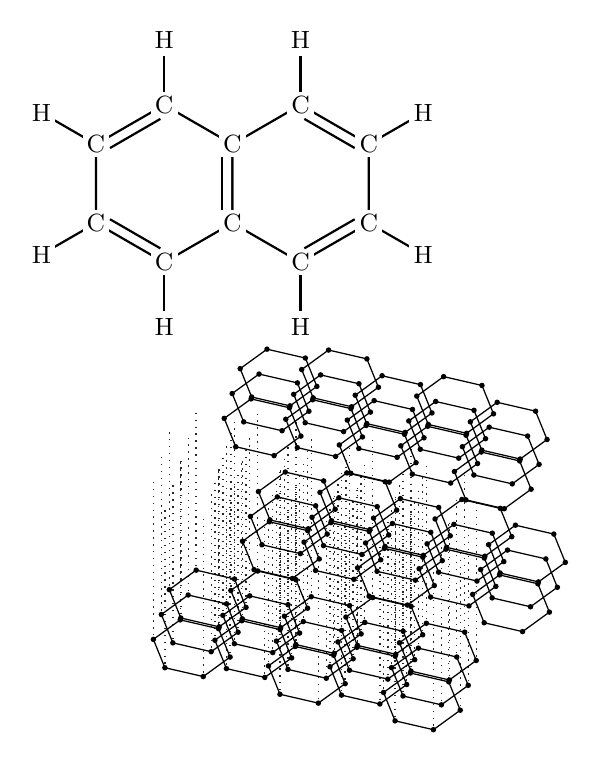
\begin{tikzpicture}[line width=0.8pt,>=Stealth]
% ---------- (a) 萘 ----------
% 六边形顶点角 30,90,...,330；左环心 (0,0)，右环心 (1.732,0)，R=1
% 环骨架
\draw (0.866,0.5) -- (0.866,-0.5) -- (0,-1) -- (-0.866,-0.5)
      -- (-0.866,0.5) -- (0,1) -- cycle;
\draw (2.598,0.5) -- (2.598,-0.5) -- (1.732,-1) -- (0.866,-0.5)
      -- (0.866,0.5) -- (1.732,1) -- cycle;
% 双键内线（向环心偏移 0.13，两端各缩短 0.13）
\draw (-0.048,0.822) -- (-0.688,0.452);   % 左环 90-150
\draw (-0.688,-0.452) -- (-0.048,-0.822); % 左环 210-270
\draw (0.736,-0.37) -- (0.736,0.37);      % 中央竖键
\draw (1.780,0.822) -- (2.420,0.452);     % 右环 90-30
\draw (2.420,-0.452) -- (1.780,-0.822);   % 右环 270-330
% H 键与 H 标记
\draw (0,1) -- (0,1.62);
\draw (0,-1) -- (0,-1.62);
\draw (-0.866,0.5) -- (-1.403,0.81);
\draw (-0.866,-0.5) -- (-1.403,-0.81);
\draw (1.732,1) -- (1.732,1.62);
\draw (1.732,-1) -- (1.732,-1.62);
\draw (2.598,0.5) -- (3.135,0.81);
\draw (2.598,-0.5) -- (3.135,-0.81);
\foreach \p in {(0,1.82),(0,-1.82),(-1.559,0.9),(-1.559,-0.9),
                (1.732,1.82),(1.732,-1.82),(3.290,0.9),(3.290,-0.9)}
  \node[fill=white,inner sep=1.5pt] at \p {\small H};
% C 原子标记（白底断线）
\foreach \p in {(0.866,0.5),(0.866,-0.5),(0,-1),(-0.866,-0.5),(-0.866,0.5),(0,1),
                (1.732,1),(2.598,0.5),(2.598,-0.5),(1.732,-1)}
  \node[fill=white,inner sep=1.5pt] at \p {\small C};
% ---------- (b) 石墨 ----------
% 局部蜂窝坐标先 y 压缩 0.72 再旋转 -13 度：wx = c*x + s*y, wy = -s*x + c2*y
% c=cos13=0.97437, s=0.22495(=0.72*sin13), c2=0.72*cos13=0.70155
\begin{scope}[shift={(0.35,-5.9)}]
% 隔层竖直虚线（顶->底，同局部点世界 x 相同）
\foreach \i in {0,1,2,3,4}
  \foreach \j in {0,1,2}
    \foreach \k in {0,1,...,5}{
      \pgfmathsetmacro{\cx}{0.75*\i}
      \pgfmathsetmacro{\cy}{0.45*(\j+mod(\i,2)*0.5)}
      \pgfmathsetmacro{\vx}{\cx+0.5*cos(60*\k)}
      \pgfmathsetmacro{\vy}{\cy+0.5*sin(60*\k)}
      \pgfmathsetmacro{\wx}{0.97437*\vx+0.22495*\vy}
      \pgfmathsetmacro{\wy}{-0.22495*\vx+0.70155*\vy}
      \draw[dotted,line width=0.5pt,black!85] (\wx,2.0+\wy) -- (\wx,\wy);
    }
% 网格线（世界坐标）
\newcommand{\graphlines}[2]{% #1=x shift, #2=y shift
  \foreach \i in {0,1,2,3,4}
    \foreach \j in {0,1,2}{
      \begin{scope}[line width=0.45pt]
        \foreach \k in {0,1,...,5}{
          \pgfmathsetmacro{\cx}{#1+0.75*\i}
          \pgfmathsetmacro{\cy}{#2+0.45*(\j+mod(\i,2)*0.5)}
          \pgfmathsetmacro{\ax}{\cx+0.5*cos(60*\k)}
          \pgfmathsetmacro{\ay}{\cy+0.5*sin(60*\k)}
          \pgfmathsetmacro{\bx}{\cx+0.5*cos(60*\k+60)}
          \pgfmathsetmacro{\by}{\cy+0.5*sin(60*\k+60)}
          \pgfmathsetmacro{\axw}{0.97437*\ax+0.22495*\ay}
          \pgfmathsetmacro{\ayw}{-0.22495*\ax+0.70155*\ay}
          \pgfmathsetmacro{\bxw}{0.97437*\bx+0.22495*\by}
          \pgfmathsetmacro{\byw}{-0.22495*\bx+0.70155*\by}
          \draw (\axw,\ayw) -- (\bxw,\byw);
        }
      \end{scope}
    }
}
% 原子黑点（世界坐标，逐层）
\newcommand{\graphdots}[2]{% #1=x shift, #2=y shift
  \foreach \i in {0,1,2,3,4}
    \foreach \j in {0,1,2}
      \foreach \k in {0,1,...,5}{
        \pgfmathsetmacro{\cx}{#1+0.75*\i}
        \pgfmathsetmacro{\cy}{#2+0.45*(\j+mod(\i,2)*0.5)}
        \pgfmathsetmacro{\vx}{\cx+0.5*cos(60*\k)}
        \pgfmathsetmacro{\vy}{\cy+0.5*sin(60*\k)}
        \pgfmathsetmacro{\wx}{0.97437*\vx+0.22495*\vy}
        \pgfmathsetmacro{\wy}{-0.22495*\vx+0.70155*\vy}
        \fill (\wx,\wy) circle (0.035);
      }
}
\graphlines{0}{0}
\graphdots{0}{0}
\graphlines{0.7}{2.0}
\graphdots{0.7}{2.0}
\graphlines{0}{4.0}
\graphdots{0}{4.0}
\end{scope}
\end{tikzpicture}
\end{document}
